\documentclass{ercisbeamer}

\title{Understanding the Brain}
\subtitle{Effective Studying}
\author{Sven Ligensa}
\institute{European Research Center for Information Systems (ERCIS)}
\date{\today}


\begin{document}

\setbgimage{00_resources/jungle_brain}
\begin{frame}
    \begin{tbox}
        \titlepage
    \end{tbox}
\end{frame}
\setbgimage{}

\begin{frame}{Contents}
    \tableofcontents
\end{frame}

\setbgimage{03_resources/neurons_50}
\section{Circuitry \& Neuroplasticity}
\begin{frame}{Circuitry \& Neuroplasticity}
    \begin{tbox}
        \begin{itemize}
            \item \red{Neurons} communicating via \red{synapses} (connection between neurons)
            \begin{itemize}
                \item Enables: Senses, cognition, motor skills, learning, memory, ...
                \item Forms possibilities and limits of person's intellectual capacity
            \end{itemize}
            \item \red{Neuroplasticity}: Brain is remarkably mutable (``plastic'')
            \begin{itemize}
                \item Learning $\Leftrightarrow$ Changing the brain
                \item Analogy: Backpropagation \grey{(used in Deep Learning)}
                \item Genes $\rightarrow$ Brain architecture (initialization point)
                \item Experience $\rightarrow$ Modification of fine structure
            \end{itemize}
        \end{itemize}
    \end{tbox}

    \begin{tbox}
        \begin{itemize}
            \item \citet{wieman12}: \red{Brain $\approx$ Muscle}
            \begin{itemize}
                \item ``The learning of \emph{complex expertise} is thus quite \emph{analogous to muscle development}. \\
                In response to the extended strenuous use of a muscle, it grows and strengthens. \\
                In a similar way, the brain changes and develops in response to its strenuous extended use.''
            \end{itemize}
        \end{itemize}
    \end{tbox}

    \begin{picture}(0,0)
        \put(359,104){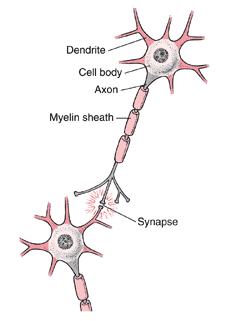
\includegraphics[width=0.179\paperwidth]{03_resources/neuron_schematic.png}}
    \end{picture}
    \begin{textblock*}{500pt}(0pt, -102pt)
        \tiny \url{https://www.researchgate.net/figure/Schematic-picture-of-two-neurons-Neurons-send-action-potentials-along-the-axon-which_fig1_41674066}
    \end{textblock*}
\end{frame}
\setbgimage{}

\section{Knowledge \& Memory}
\begin{frame}{Knowledge \& Memory}
    \begin{itemize}
        \item \red{Knowledge} and \red{memory} = Neural processes
        \begin{itemize}
            \item Maturation of connections = Gradual thickening of myelin coating of axons
            \item Practice $\Rightarrow$ Myelin $\uparrow$ $\Rightarrow$ Strength and speed of electrical signals $\uparrow$ \\ $\Rightarrow$ Performance $\uparrow$ ($\Rightarrow$ Motivation for further practice)
        \end{itemize}
        \item Actions taken by \red{habit} are directed from region located deeper in the brain
        \begin{itemize}
            \item Chunk sequence of steps to single unit $\Rightarrow$ Sequence becomes reflexive
            \item Examples: Finger movement of musicians, typing on a keyboard
            \item Analogy: Computer macro
        \end{itemize}
    \end{itemize}
\end{frame}

\setbgimage{03_resources/working_memory_50}
\section{IQ \& Working Memory}
\begin{frame}{IQ \& Human's Working Memory}
    \begin{tbox}
        \begin{itemize}
            \item \red{IQ}
            \begin{itemize}
                \item Determined by genes and environment $\Rightarrow$ \red{Not fixed}
                \item Fluid intelligence (abstract reasoning) vs. Crystallized intelligence (concrete knowledge)
            \end{itemize}
            \item Human's \red{Working Memory}
            \begin{itemize}
                \item Amount of information that can be held in mind while working through a problem
                \item Analogy: RAM in a computer
                \item \negative{Severely limited}, correlates with IQ
                \item \positive{Positive attitude towards learning} $\Rightarrow$ Better use of working memory
            \end{itemize}
        \end{itemize}
    \end{tbox}
\end{frame}
\setbgimage{}

\section*{Outlook}
\begin{frame}{Outlook}
    \begin{enumerate}
        \item \positive{Introduction}
        \vspace{.5em}
        \item \positive{Illusions of Knowing}
        \item \positive{Understanding the Brain}
        \item Next: \red{Learning}
        \item \grey{Desirable Difficulties}
        \item \grey{Effective vs. Ineffective Learning Strategies}
        \vspace{.5em}
        \item \grey{Retrieval}
        \item \grey{Spacing}
        \item \grey{Variation and Interleaving}
        \item \grey{Mental Models}
        \item \grey{Memory Cues}
    \end{enumerate}
\end{frame}

\thankyou{Happy Learning!}{sven.ligensa@uni-muenster.de}

\sources

\end{document}
